\subsection{System Experiments}\label{subsec:expsystem}
An important aspect of the experiments, is to validate if there is an impact on tripscores caused by the diversity of users' smartphones. In a usage-based insurance context, users needs to be treated equally, which relies entirely upon their smartphone and the GPS antenna. Two smartphones logging the same trip, should report the same tripscore. Such an analysis can be quite extensive, involving an entire market of smartphones and different versions of GPS antennas. Instead, a small initial test with a selection of different smartphones will tell whether this system is vulnerable to GPS inaccuracy. 

This small initial test will be referred to as an applicability test. An applicability test will confirm whether or not smartphones are good enough to equally score trips. It was conducted by bringing five different smartphones and two high quality GPS trackers\citep{quality_gps_device} into the same car, and recording the trip with all entities at the same time. If the system is applicable for usage-based insurance, the smartphones needs to report the same tripscores, and the route needs to be highly similar to those recorded by the high quality GPS trackers.
 
\begin{figure}[tb]
\centering
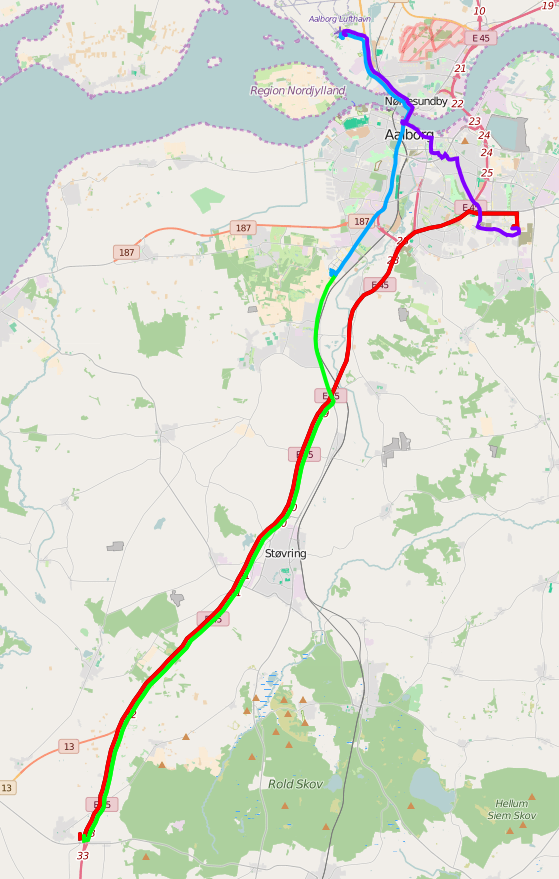
\includegraphics[width=0.465\textwidth]{Pictures/experiment_routes}
\caption{Routes traveled in the area of Aalborg during the experiment}
\label{fig:experiment_routes}
\end{figure}

With these seven devices, four trips were completed driving around in northern Jutland, in the vicinity of Aalborg. Raw data from the trips can be seen in Tables \ref{exp1trip1}, \ref{exp1trip2}, \ref{exp1trip3} and \ref{exp1trip4} in Appendices. A summary of the tripscores for each phone, during the four trips, can be seen in Table \ref{tab:smartphone_test_one}.

\begin{table*}[tb]
\centering
\caption{The tripscores from all seven recording devices, on all four trips used, during the first test}
\label{tab:smartphone_test_one}
\begin{tabular}{|l|llll|}
\hline
\rowcolor{tablegreen}

                   & \textbf{Trip 1}    & \textbf{Trip 2}    & \textbf{Trip 3}    & \textbf{Trip 4}  \\\hline
OnePlus One        & 50.191   & \ \  58.922   & 42.751   & 23.228 \\
Samsung Galaxy S5  & 40.092   & \ \ 56.781   & 24.026   & 27.530 \\
HTC One Mini 2     & 75.063   & \ \ 28.734   & 21.012   & 19.203 \\
Huawei Y330        & 81.819   &  128.056   & 50.622   & 13.082 \\
Samsung Galaxy S4  & 37.010   & \ \ 27.762   & 16.927   & 18.825 \\
BT-Q1300ST (\#1)   & 37.910   & \ \ 25.373   & 20.981   & 23.917 \\
BT-Q1300ST (\#2)   & 69.956   & \ \ 72.785   & 85.139   & 27.074 \\\hline

\end{tabular}
\end{table*}

When examining trip 1 from Table \ref{tab:smartphone_test_one} which has a length of approximately 36.200 meters, two smartphones and one high quality GPS gets a score ranging from 37.000-40.000 which is good. But the remaining four tripscores disagree with varying severity. The worst is the Huawei Y330, which score this trip 81.819. However, the Huawei Y330 only logs 23\% of the average GPS coordinates compared to the other devices. The Huawei continues this trend throughout the test, and seems unfit for use in usage-based insurance. Another alarming result in trip 1 is the degree to which the two high quality GPS devices disagrees. One scores the trip 37.910 and the other 69.956 which is a big difference.

Looking at trip 2 in Table \ref{tab:smartphone_test_one} which has a length of approximately 28.200 meters, three devices range from 25000-28750 in tripscore. The noteworthy result compared to trip 1 is, that the three devices with a low tripscore are not the same as those in trip 1.

The same pattern reoccur with trip 3 from Table \ref{tab:smartphone_test_one}, which has a length of approximately 13.400, but this time four devices gets a score ranging from 16.500-24.050, which are rather similar. The last three devices got a much higher tripscore, the highest being 85.139, approximately 535\% above the trip-length, and it was logged by one of the high quality GPS devices. To highlight the disagreement between the two high quality GPS devices, the other device got a score of 20.981. 

The pattern is broken with trip 4 from Table \ref{tab:smartphone_test_one}, where all devices range between 13.000-27.550. This may still be somewhat diversified scores, but to compare it to trip 3, the highest device only scored approximately 91\% above the trip-length from this trip, compared to 535\% in trip 3. The two high quality GPS devices also fairly agrees on the tripscore for trip 4, 23.917 and 27.075 respectively. 

When analyzing the results from this test, the immediate thought may be to throw away the smartphone as usage-based insurance component. Concern about accuracy, integrity, availability and continuity of service in standalone GPS receivers is also raised in \citep{art:challenges_smartphone_ubi} \citep{art:survey_mobile_phone_sensing} \citep{art:smartphones_for_monitoring_and_ubi} \citep{art:insurtelematics} \citep{art:in-car_positioning_technologies}. But two other factors may have influenced the results in Table \ref{tab:smartphone_test_one}. The first factor is GPS interference, in which case the test setup could have changed the results, because all the GPS devices was kept close together in a fabric container and placed in the front of the car near the windshield. This could affect the GPS receivers by interfering with each other \citep{art:gps_interference_two} \citep{art:gps_interference_one}. This position was decided upon, because a common reference point was valued in the applicability test. One article provides concrete results in terms of coverage from smartphone GPS receivers, and during an 1 hour and 15 minutes trip, 6 heavy brakes was detected with an OBD device inside the car. A total of seven smartphones was brought on this trip, and they had a coverage in the interval of 60\% to 99.7\% when detecting these brakes \citep{art:insurtelematics}, which states they are indeed vulnerable to inaccuracy. Coverage means the degree to which the smartphones align with the control-unit, in this case the OBD. The test also included outliers, false positives, and indeterminable which causes the percentages to be skewed.

The second factor is the use of third party software for map-matching of the spatio-temporal trajectories collected by the smartphones, called TrackMatching \citep{trackmatch}. TrackMatch attempts to map-match a series of spatio-temporal points to the OSM road network, and output the entire route by segments and map-adjusted GPS points. How TrackMatch decides to readjust these GPS points are uncontrollable for this system, and no module was implemented to oversee this readjusting, so this influence cannot be changed.

It was decided to repeat the applicability test and eliminate the GPS interference as much as possible. The GPS devices was arranged in the car with as much distance as possible between them. The possible margin of error by using a separated reference point was disregarded. The Huawei Y330 was also omitted. 

\begin{table*}[tb]
\centering
\caption{The tripscores from all six recording devices, on all four trips used, during the second test}
\label{tab:smartphone_test_two}
\begin{tabular}{|l|llll|}
\hline
\rowcolor{tablegreen}

                   & \textbf{Trip 1}    & \textbf{Trip 2}    & \textbf{Trip 3}    & \textbf{Trip 4}  \\\hline
OnePlus One        & 64.511  & 31.075  & 17.103  & 18.223 \\
Samsung Galaxy S5  & 46.668  & 48.169  & 19.010  & 22.779 \\
HTC One Mini 2     & 54.564  & 39.439  & 27.674  & 29.767 \\
Samsung Galaxy S4  & 37.475  & 29.242  & 16.672  & 18.094 \\
BT-Q1300ST (\#1)   & 37.800  & 30.397  & 26.440  & 25.064 \\
BT-Q1300ST (\#2)   & 41.260  & 37.029  & 36.531  & 45.327 \\\hline

\end{tabular}
\end{table*}

The test results shown in Table \ref{tab:smartphone_test_two} once again shows a considerable difference when comparing the two high quality GPS devices. But the difference is decreased substantially compared to the first test, which signifies that some external influence may have been affecting the devices. Looking at the raw data in Tables \ref{exp1trip1} through \ref{exp2trip2}, an observation is that their behavior is consistent. When looking at the amount of accelerations, brakes and jerks, one device consistently counts more than the other. BT-\#1 counted a total of 1529 of these events, whereas BT-\#2 counted a total of 3894. That is 191.13 events per trip on average for BT-\#1, and 486.75 events per trip on average for BT-\#2. This generalization of more events registered by BT-\#2 are present in both tests. This signifies that it may not be able to conclude any comparison between these two devices, because they deliver such different results.

The results from Samsung Galaxy S4, Samsung Galaxy S5 and BT-\#1 from the second test, actually compares well to the results they provided in the first test. There is an influence in the driving style, but both tests was performed by the same driver. The driver attempted to follow his personal driving style during both tests. Additionally, traffic may also influence the results in the tests, but the tests was performed in a similar time-period, both on a weekday. 

The remaining devices disagrees with their results from the first test to the second test, for atleast some of the trips. When looking at the overall result from both tests, the system is not currently applicable for usage-based insurance. This is due to the diversity in tripscores for similar trips, making it unfair to the policyholders. However, several articles raised concern about the GPS receivers, but some also suggested a way of supporting the raw data with model-based signal processing and an outlier rejection scheme \citep{art:challenges_smartphone_ubi} \citep{art:smartphones_for_monitoring_and_ubi} \citep{art:insurtelematics}. This would make the trajectories more stringent, and possibly eliminate falsely positive delinquencies caused by a jumpy GPS coordinate. It is considered a good next step to design and implement such a scheme in the system. This scheme could make each GPS receiver agree more with itself. If it could be achieved that every GPS device produces reproducible results, a calibration mechanism could eliminate the diversity caused by different GPS devices. This would ultimately cleanse the instability about accuracy, integrity, availability and continuity of service from standalone GPS receivers, and make the system robust enough to apply entirely to usage-based insurance.

\subsection{Pearson Correlation}\label{subsec:pearsoncorrelation}

In order to test the validity of our metrics and the chosen policy, a the pearson correlation between the metrics have been conducted. The point of the test is to make sure no metrics are directly correlating, meaning one of the metrics is negligible. There is a number of different reasons as to why the outcome will look as it does, and it will be discussed thoroughly. The Pearson-Correlation have been calculated on the individual scores given to a trip per each of metrics. 

The matrix of pearson correlations between the metrics is shown at table \ref{tab:pearsonmatrix}. The most notable result is the multicollinearity between accelerations and brakes, which seems rather odd as they are diametrical opposites and can per definition not exist at the same time. Another highly correlating metric is jerks having a correlation of 0.828 with both brakes and accelerations. 

\begin{table*}[tb]
\centering
\caption{This is the pearson correlation matrix between the metrics}
\label{tab:pearsonmatrix}
\begin{tabular}{l|llllll}
                      & Roadtypes & Critical Time Periods & Speeding & Accelerations & Brakes & Jerks  \\ \hline
Roadtypes             & 1         & -0.250                & -0,546   & -0.341        & -0,348 & -0,241 \\
Critical Time Periods & -0.250    & 1                     & 0.156    & 0.460         & 0.428  & 0.313  \\
Speeding              & -0,546    & 0.156                 & 1        & 0.196         & 0.195  & 0.144  \\
Accelerations         & -0.341    & 0.460                 & 0.196    & 1             & 0.971  & 0.828  \\
Brakes                & -0,348    & 0.428                 & 0.195    & 0.971         & 1      & 0.828  \\
Jerks                 & -0,241    & 0.313                 & 0.144    & 0.828         & 0.828  & 1     
\end{tabular}
\end{table*}

Looking closer at the multicollinearity between accelerations and brakes, there is a couple of different factors which affect the result. As mentioned accelerating and braking are diametrically opposite, but they are both dependant of the speed of the vehicle (as they are calculated through the change in speed). If the driver performs a big acceleration, his speed is high and he at some point needs to brake in order to decline in speed. 

\begin{figure}[tb]
\centering
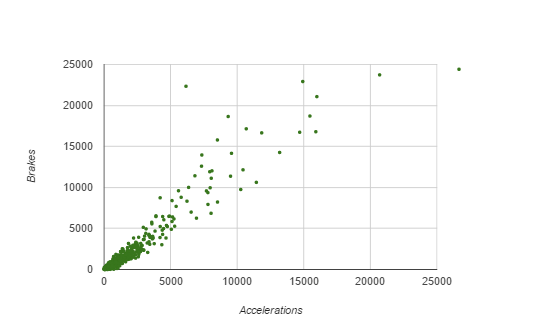
\includegraphics[width=0.465\textwidth]{Pictures/abcorrel}
\caption{The correlation between accelerations and brakes}
\label{fig:abcorrel}
\end{figure}

The figure shown at \ref{fig:abcorrel} clearly illustrates the correlation. Another reasoning as to why these metrics correlate can be the thresholds in the policy used to calculate the scores. As earlier mentioned the threshold for brakes are 8 $m/s^2$ whereas accelerations are counted from 5 $m/s^2$. If we had no thresholds and the delinquencies were scored the same, the correlation would be 1.0 as it only depended on the speed of the vehicle. 
Jerks was the metric met with the highest level of scepticism when implemented, and the correlation shows that it was not completely unwarranted. It does show a lot of correlation with both brakes and accelerations. The figure \ref{fig:ajcorrel} shows the correlation between accelerations and jerks. Jerks are as mentioned calculated as $m/s^3$, and a driver with many accelerations are almost bound to have a lot of jerks as it is hard to keep a constant acceleration.

\begin{figure}[tb]
\centering
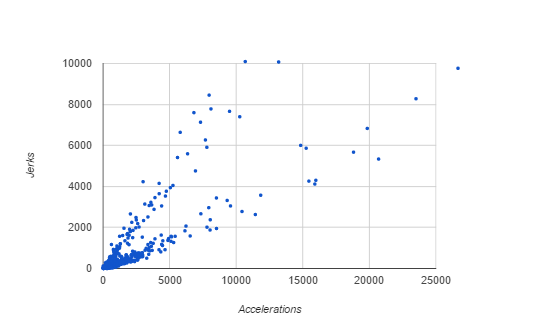
\includegraphics[width=0.465\textwidth]{Pictures/ajcorrel}
\caption{The correlation between accelerations and jerks}
\label{fig:ajcorrel}
\end{figure}


the similar correlation between the two can be answered by the correlation between accelerations and brakes. 


\subsection{Driver Profiling}\label{subsec:userprofiling}

Creating driver profiles is one of the strengths in Drive-LaB. With a descriptive set of metrics it is possible to differentiate between drivers, and create fairly accurate driver profiles without compromising the users privacy. The entire concept of a driver profile is relevant for this project due to the direct connection to the insurance industry. Naturally, it is possible to evaluate the drivers insurance costs more precisely, if the given driver profile is accurate. However driver profiles is demanded to be accurate and portray the full picture when you are dealing with paying customers\citep{art:insurtelematics} -as they need an incentive to use the product. In the remainder of this section, two random driver profiles will be reviewed and used to illustrate the capabilities in Drive-LaB to differentiate between styles of driving.  

\paragraph{Score Percentages} are a great way to differentiate between drivers. The two drivers will be referenced to as Driver 1 with an average tripscore percentage of 65,08\%, and Driver 2 with an average tripscore percentage of 39,07\%.

Beside the obvious difference in percentages, looking at where the drivers generate their scores show clear differences. Figure \ref{fig:avgmetricper} and Figure \ref{fig:piecharts} shows a comparison between the two drivers, portrayed as a bar chart and a pie chart with the distribution of the tripscore based on metrics. Looking at Driver 1, a lot of the score actually comes from accelerations at roughly 21\%, brakes at roughly 28\% and to some extend jerks at roughly 11\%. It is also worth mentioning that roadtypes actually scored negative on average. Looking at the pie chart in Figure \ref{fig:piecharts}, brakes is easily recognizable as the biggest contributor to a higher score.

\begin{figure*}[tb]
\centering
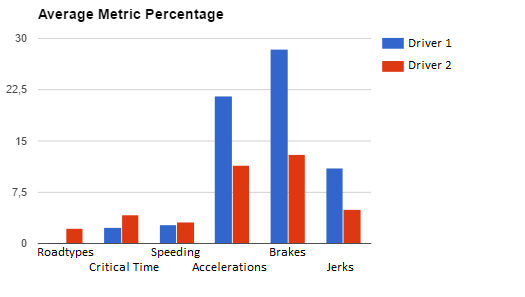
\includegraphics[width=0.465\textwidth]{Pictures/AverageMetricsPercentage}
\caption{A bar chart of the distribution of tripscore percentage by metrics for Driver 1 and Driver 2}
\label{fig:avgmetricper}
\end{figure*}

\begin{figure*}[tb]
\centering
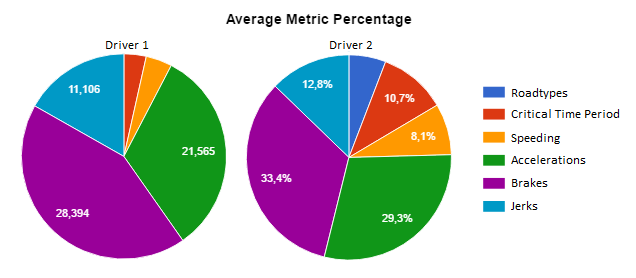
\includegraphics[width=0.95\textwidth]{Pictures/piecharts}
\caption{A bar chart of the distribution of tripscore percentage by metrics for Driver 1 and Driver 2}
\label{fig:piecharts}
\end{figure*}

Driver 2 has quite a different distribution than Driver 1, aside from a lower tripscore percentage in general. Accelerations and brakes clearly heavily influence the score in the system, however this driver have a significantly lower percentage in both of the metrics in the tripscore. This is noticeable in the pie chart in Figure \ref{fig:piecharts} which shows far less disparity between the metrics than the previous driver. 

\paragraph{Normalized Metrics} are the average metrics on a certain distance driven. For easy comparison the distance chosen is 1.000 meters. Looking at Driver 1, in Figure \ref{fig:avgmetricnorm}, Driver 1 has 6.84 points with jerks flagged given the chosen distance. Looking at Driver 2 and comparing it to Driver 1, Driver 2 nearly has half the amount of accelerations, brakes and jerks per 1.000 meters. The only metric Driver 2 has more of, given the chosen distance, is speeding.

\begin{figure}[tb]
\centering
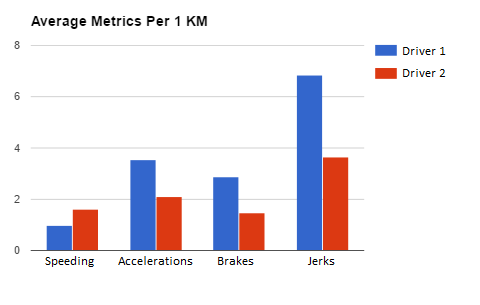
\includegraphics[width=0.465\textwidth]{Pictures/AverageMetricsNorm}
\caption{A bar chart of the metrics per 1.000 meters for Driver 1}
\label{fig:avgmetricnorm}
\end{figure}

\paragraph{Severity of Delinquencies} is one of the big tells when differentiating between drivers. It is noticeable when looking at Figure \ref{fig:car8intervals}, which represents Driver 1, there is a slight decline with a spike in the last interval. There might be several reasons as to why the last interval spike but the primary reason is that the interval is everything above a threshold, thus a much larger interval than the previous. Comparing Driver 1 to Driver 2, shown in Figure \ref{fig:car21intervals}, there is quite a different distribution.

\begin{figure*}[tb]
\centering
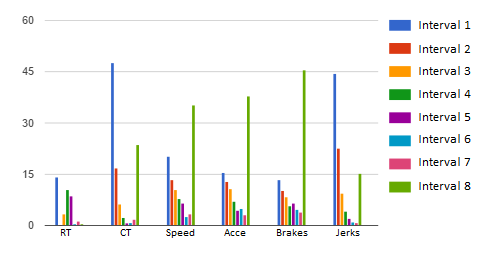
\includegraphics[width=0.95\textwidth]{Pictures/car8intervals}
\caption{A bar chart of the distribution of metrics within the intervals for Driver 1}
\label{fig:car8intervals}
\end{figure*}

\begin{figure*}[tb]
\centering
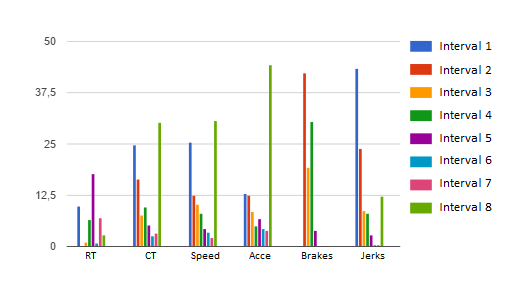
\includegraphics[width=0.95\textwidth]{Pictures/car21intervals}
\caption{A bar chart of the distribution of metrics within the intervals for Driver 2}
\label{fig:car21intervals}
\end{figure*}

It is possible to distinguish between drivers, and even more important, it is possible to create driver profiles. Given a arbitrary trip it would be possible to draw similarities between the trip and the driver profiles. From an usage-based insurance point of view, it would be possible to access the risk of a given driver. As an example, a driver with a higher amount of braking delinquencies, all represented as brakes with a hard degree, might have a higher risk of crashing and get a more expensive insurance claim.